\section{Additional information}

\begin{table}[h]
  \begin{center}
    \centering
    \begin{tabular}{@{}lllll@{}}
      \toprule
      Name        & Author              & URL (if available) \\ \midrule
      Tetris      & Felix Schoeller     &             -  \\
      Raytracer   & Alex Quach          & https://github.com/aquach/from-nand-to-raytracer   \\
      GASchunky   & Gavin Stewart       & https://github.com/gav-/Nand2Tetris-Games\_and\_Demos  \\
      GABoing     & Gavin Stewart       & https://github.com/gav-/Nand2Tetris-Games\_and\_Demos  \\
      Hackenstein & Quester Zen         & https://github.com/QuesterZen/hackenstein3D  \\
      Doom        & Jona Leon Heywinkel &             -  \\
      *Raycaster  & Julius Armbrüster   &             -  \\
      Axis        & Markus Brenneis     &             -  \\
      Brainhack   & Markus Brenneis     &             -  \\
      Minesweeper & Patrick Müller      &             -  \\ \bottomrule
    \end{tabular}
    \small
    \item The project by Julius Armbrüster did not have a name, so Raycaster was chosen to describe it
    \caption{The VM programs tested on the new emulator implementation.}%
    \label{table:tested}
  \end{center}
\end{table}

\begin{table}[h]
  \begin{center}
    \centering
    \begin{tabularx}{\textwidth}{|l|X|X|}
      \toprule
      Segment        & Purpose              & Comments \\ \midrule
      argument     & Stores the function's arguments    & Allocated dynamically by the VM implementation when the function is entered.  \\ \midrule
      local     & Stores the function's local variables  & Allocated dynamically by the VM implementation and initialized to 0’s when the function is entered.  \\ \midrule
      static     & Stores static variables shared by all functions in the same .vm file.  & Allocated by the VM imp. for each .vm file; shared by all functions in the .vm file.  \\ \midrule
      constant     & Pseudo-segment that holds all the constants in the range 0...32767.  & Emulated by the VM implementation; Seen by all the functions in the program.  \\ \midrule
      this, that     & General-purpose segments. Can be made to correspond to different areas in the heap. Serve various programming needs.  & Any VM function can use these segments to manipulate selected areas on the heap.  \\ \midrule
      pointer     & A two-entry segment that holds the base addresses of the this and that segments.  & Any VM function can set pointer 0 (or 1) to some address; this has the effect of aligning the this (or that) segment to the heap area beginning in that address.  \\ \midrule
      temp     & Fixed eight-entry segment that holds temporary variables for general use.  & May be used by any VM function for any purpose. Shared by all functions in the program.  \\
      \bottomrule
    \end{tabularx}
    \caption{Every memory segment the Hack bytecode, taken from~\cite{nisan2005}.}
    \label{table:segments}
  \end{center}
\end{table}

\cref{table:segments} was taken directly from the book accompanying the Nand to Tetris course~\cite{nisan2005}.

\begin{table}[h]
  \begin{center}
    \centering
    \begin{tabularx}{\textwidth}{|l|X|X|}
      \toprule
      Dependency        & Purpose              \\ \midrule
      lazy\_static      & Use statics with runtime initialization code. For example lookup hashmaps \\ \midrule
      regex      & Regular expressions in rust for simple parsing tasks \\ \midrule
      wasm-bindgen      & Generate JS bindings for Wasm code compiled from Rust \\ \midrule
      web-sys      & JS standard library bindings for Rust \\ \midrule
      console\_error\_panic\_hook      & Print the stack trace of a rust panic to the JS console \\ \midrule
      wasm-pack      & CLI to compile Rust to Wasm easier. Not a runtime dependency, just compile time \\ \midrule
      SDL2      & GUI framework. Originally for C, but also usable from Rust \\ \midrule
      Clap      & Parse CLI arguments \\
      \bottomrule
    \end{tabularx}
    \caption{Every dependency of the project.}
    \label{table:dependencies}
  \end{center}
\end{table}

\begin{center}
  \begin{figure}[ht]
    \centering
    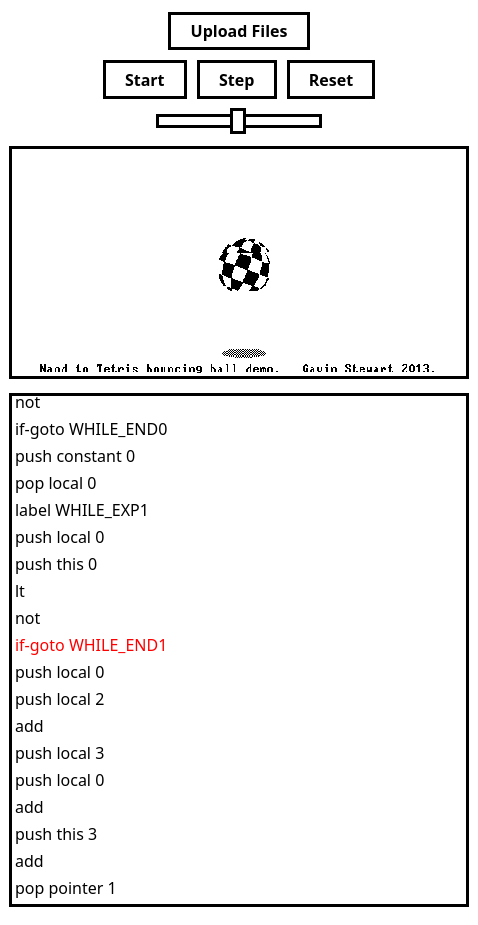
\includegraphics[width=8cm]{fig/ui-demo-mobile.png}
    \caption{The web-based user interface in a phone format.}%
    \label{fig:ui-demo-mobile}
  \end{figure}
\end{center}
% Hier können Sie Ihren Anhang definieren.

% Achten Sie darauf, dass der Anhang in Ihrer \texttt{thesis.tex}
% initial auskommentiert ist.
% Der entsprechende Part befindet sich nahe dem Ende der Datei.
% Entfernen Sie bei Bedarf die Kommentierung um den Anhang nutzen zu können.


% \section{Nutzung}

% Der Anhang wird wie die Abschnitte des Hauptteils der Arbeit gestaltet,
% also mit \texttt{\textbackslash section} Befehlen.

% \subsection{Unterabschnitte}
% Die Verwendung von Unterabschnitten im Anhang
% mittels \texttt{\textbackslash subsection}
% funktioniert ebenfalls!
